% use "pdflatex -output-directory=../output Math-Notes.tex" to compile for git (assuming your in . directory)
\documentclass{report}

\input{preamble}
\input{macros}
\input{letterfonts}

\title{\Huge{Math}\\Notes}
\author{\huge{By me (Thanks to for the template \href{https://github.com/SirCharlieMars/dotfiles/tree/master/latex_template}{SirCharlieMars})}}
\date{}

\begin{document}

\maketitle
\newpage% or \cleardoublepage
% \pdfbookmark[<level>]{<title>}{<dest>}
\pdfbookmark[section]{\contentsname}{toc}
\tableofcontents


\pagebreak % 1.1


\chapter{Algebra}
\section{Indices}
\gls{test}{test1}

\dfn{Index Laws}{
    \begin{enumerate}
        \item $a^m \times a^n = a^{n + m}$
        \item $a^m \div a^n = a^{n - m}$
        \item $(a^m)^n = a^{m \times n}$
        \item $a^{-m} = \frac{1}{a^m}$
        \item $a^0 = 1$
        \item $a^{\frac{m}{n}} = \sqrt[n]{a^m}$
    \end{enumerate}
}

\ex{Laws In Action}{
    \begin{enumerate}
        \item $2^3 \times 2^7 = 2^{10}$
        \item $\frac{3^6}{3^2} = 3^4$
        \item $(5^2)^5 = 5^{10}$
        \item $7 \times 2^{-2} = \frac{7}{2^2}$
        \item $45^0 = 1$
        \item $5^{\frac{-3}{7}} = \frac{1}{\root 7 \of {5^3}}$
    \end{enumerate}
}
\nt{Indices are used extremely frequently and there are often multiple laws hidden in each question}


\pagebreak


\section{Logarithms (Logs)}

\dfn{Principle}{The general equation is: \[log_{(a)}(y) = x \leftrightarrow a^x = y\]\\For example:\[log_{10}1 = 0 \leftrightarrow 10^0 = 1\]\\To calculate logarithm: \[\frac{log_{10}y}{log_{10}a}\]}
\dfn{Laws}{
    \begin{enumerate}
    %% contains in and out of brackets
        \item $\log_{a}x + \log_{a}y = \log_{a}xy$
        \item $\log_{a}x - \log_{a}y = \log_{a}\frac{x}{y}$
        \item $\log_{a}x^n = n\log_{a}x$
        \item $\log_{a}a = 1$
        \item $\log_{a}1 = 0$
    \end{enumerate}
    To use these laws, the bases must be the same $a$
}

\ex{Laws In Action}{Round to two decimal place
    \begin{enumerate}
        \item $\log_{2}2 + \log_{2}5 = \log_{2}10 = 3.32$
        \item $\log_{5}12 - \log_{5}2 = \log_{5}6 = 1.11$
        \item $\log_{7}{2^2} = 2 \times \log_{7}2 = 0.71$
        \item $\log_{84}84 = 1$
        \item $\log_{153}1 = 0$
    \end{enumerate}
}

\nt{some calculators have a default log base of 10, this means $\log_{10}(x) = \log_{}(x)$}


\pagebreak


\section{Quadratic Equations}

\dfn{Formulae}{A quadratic equation is an equation where the highest power is two.\\The standard form quadratic equation: \[ax^2 + bx + c = 0\] where $a,b,c$ are known.\\The quadtratic formula (can only be used by standard form equations):\[x = \frac{-b \pm \sqrt{b^2-4ac}}{2a}\]\\Completing the square \[ax^2 + bx + c = 0\rightarrow \]\\The porabola:\[y = ax^2 + bx + c\]}


\chapter{Trigonometry}
\section{Right-Angled}
\dfn{Identification}{A triangle is right-angled if it contains a right angle ($90^\circ$):\[
\begin{tikzpicture}
    \draw [line width=1.5pt, fill=gray!2] (0,0) -- (0:3) -- (4,0) -- cycle;

    \coordinate[label=left:$$]  (A) at (0,0);
    \coordinate[label=right:$$] (B) at (4,0);
    \coordinate[label=above:$$] (C) at (0,3);

    \coordinate[label=below:$c$](c) at ($ (A)!0.5!(B) $);
    \coordinate[label=left:$b$] (b) at ($ (A)!0.5!(C) $);
    \coordinate[label=right:$a$](a) at ($ (B)!0.5!(C) $);

    % right angle
    \draw (0cm,0cm) rectangle (0.5cm,0.5cm);

    % angle beta
    \begin{scope}[shift={(4cm,0cm)}]
        \draw[fill=green!30] (0,0) -- (-180:0.75cm) arc (180:120:0.45cm);
        \draw (162:1cm) node {$\theta$};
    \end{scope}

    % the triangle
    \draw [line width=1.5pt] (A) -- (B) -- (C) -- cycle;
\end{tikzpicture}
\]
}
\dfn{Formulae}{Pythagorean theorem $c^2 = a^2 + b^2$ can find the exact length of the an unknown side given two other known sides.\\\\The Area Formula $A = \frac{1}{2}bh$ is used to find the area of the right angle triangle}
% Add examples
\dfn{Trigonometric Ratios}{Trigonometric Ratios are ratios that can find angles and sides of a right-angled triangle:\\\\Sine:\[\sin\theta = \frac{o}{h}\]\\Cosine:\[\cos\theta = \frac{a}{h}\]\\Tangent:\[\tan\theta = \frac{o}{a}\]\\$\theta$ can be found with Inverse Ratios.\\\[\theta = \sin^{-1}{\frac{o}{h}}\]\[\theta = \cos^{-1}{\frac{a}{h}}\]\[\theta = \tan^{-1}{\frac{o}{a}}\]}
% Add examples
\nt{To remember the Trigonometric ratios, we can use $SOHCAHTOA$.} % SOHCAHTOA explanation later

% Add examples
\pagebreak

\section{Non-Right-Angled}
\dfn{Identification}{A triangle is non-right-angled if it does not contain a right angle ($90^\circ$)\\\\The general rule for keeping sides and angles uniform in a non-right-angled triangle is:
\[
    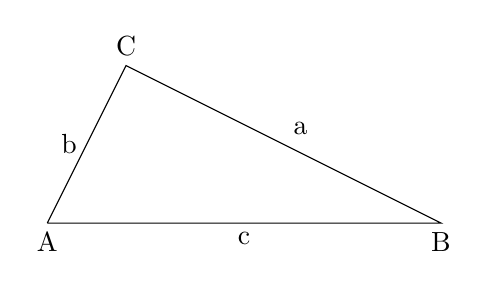
\begin{tikzpicture}
        \draw  (-1, 0) coordinate (A)
        -- node[left] {b} (0,2) coordinate (c)
        -- node[above right] {a} (4,0) coordinate (b)
        -- node[below] {c}  (-1, 0) coordinate (a);
        \node at (a)[anchor=north] {A};
        \node at (b)[anchor=north] {B};
        \node at (c)[anchor=south] {C};
    \end{tikzpicture}
\]
The area can be found with the Area Forumla $A = \frac{1}{2}ab\sin{C}$
}
\dfn{Sine Rule}{The Sine Rule allows for angles and sides to be found within a non-right-angled triangle. To find a side using the Sine Rule, use:\\\[\frac{a}{\sin{A}} = \frac{b}{\sin{B}} = \frac{c}{\sin{C}}\]\\To find an angle using the Sine Rule, use:\\\[\frac{\sin{A}}{a} = \frac{\sin{B}}{b} = \frac{\sin{C}}{c}\]}
\nt{Using the Sine Rule requires two known sides/angles and a known side/angle}
% Add examples
\dfn{Cosine Rule}{Like the Sine Rule, the Cosine Rule allows for angles and sides to be found within a non-right-angled triangle. The Cosine Rule is:\\\[c^2 = a^2 + b^2 -2ab\cos{C}\]\\And to find an angle:\[\cos{C} = \frac{a^2 + b^2 - c^2}{2ab}\]}

\pagebreak

\section{Exact Triangles}
\dfn{Identification}{Exact Triangles are triangles that have exect trigonometric values for specific angles. \[
\begin{tikzpicture}
    \draw [line width=1.5pt, fill=gray!2] (0,0) -- (0:3) -- (4,0) -- cycle;

    \coordinate[label=left:$$]  (A) at (0,0);
    \coordinate[label=right:$$] (B) at (3,0);
    \coordinate[label=above:$$] (C) at (0,4);

    \coordinate[label=below:$1$](c) at ($ (A)!0.5!(B) $);
    \coordinate[label=left:$\sqrt{3}$](b) at ($ (A)!0.5!(C) $);
    \coordinate[label=right:$2$](a) at ($ (B)!0.5!(C) $);

    % right angle
    \draw (0cm,0cm) rectangle (0.5cm,0.5cm);

    % angle 60
    \begin{scope}[shift={(4cm,0cm)}]
        \draw[fill=green!30] (-1,0) -- (-180:1.75cm) arc (180:120:0.65cm);
        \draw (162:1cm) node {$60$};
    \end{scope}

    % % angle 30
    \begin{scope}[shift={(0.7cm,4cm)}]
        \draw[fill=blue!30] (0,0) -- (-180:0.75cm) arc (180:120:0.45cm);
        \draw (162:1cm) node {$30$};
    \end{scope}

    % the triangle
    \draw [line width=1.5pt] (A) -- (B) -- (C) -- cycle;
\end{tikzpicture}
\]}

% TODO: surds



\end{document}
